\section{Schedule}\label{sec:schedule}
In this section the schedule for the \emph{PowerEnJoy project} will be presented; it is a high-level general schedule that allows the reader to understand the main phases of the project specification and development.

\subsection{Notes for the charts}
\subsubsection{\hyperref[fig:rasdGantt]{RASD Gantt chart}}
\begin{itemize}
	\item \textbf{Meetings with client}: all the resources will be present at the meeting
	\item \textbf{Modelization of the World and the Machine}: this part requires discussion and cooperation, hence it will be assigned to all the resources
	\item \textbf{Identification of use cases}: Davide will start working on this activity in date 28/10/2016
	\item \textbf{In progress meeting with client}: all the resources will be present at the meeting
	\item \textbf{Requirements refinement}: the requirements will be updated based on updates made in other parts of the document, during its development
	\item \textbf{Alloy modelization}: Davide will start working on this activity in date 05/11/2016
	\item \textbf{Document revision}: these days are left for the revision of the document and to complete tasks that eventually need more time
\end{itemize}

\subsubsection{\hyperref[fig:ddGantt]{DD Gantt chart}}
\begin{itemize}
	\item \textbf{Architecture draft}: this part requires discussion and cooperation, hence it will be assigned to all the resources
	\item \textbf{Meeting with clients}: all the resources will be present at the meeting
	\item \textbf{Sequence diagrams}: Moreno will start working on this activity in date 29/11/2016
\end{itemize}

\subsubsection{\hyperref[fig:itpdGantt]{ITPD Gantt chart}}
\begin{itemize}
	\item \textbf{Integration test strategy and Definition of precedences}: these initial tasks will be accomplished at the same time and since they requires discussion and cooperation, they will be assigned to all the resources
	\item \textbf{Document revision}: Davide will start working on this activity in date 19/12/2016
\end{itemize}

\subsubsection{\hyperref[fig:devGantt]{Development Gantt chart}}
All of the tasks in this chart refers to high level activities; more specific charts will be produces during the development phase.

\begin{figure}[h]
	\centering
	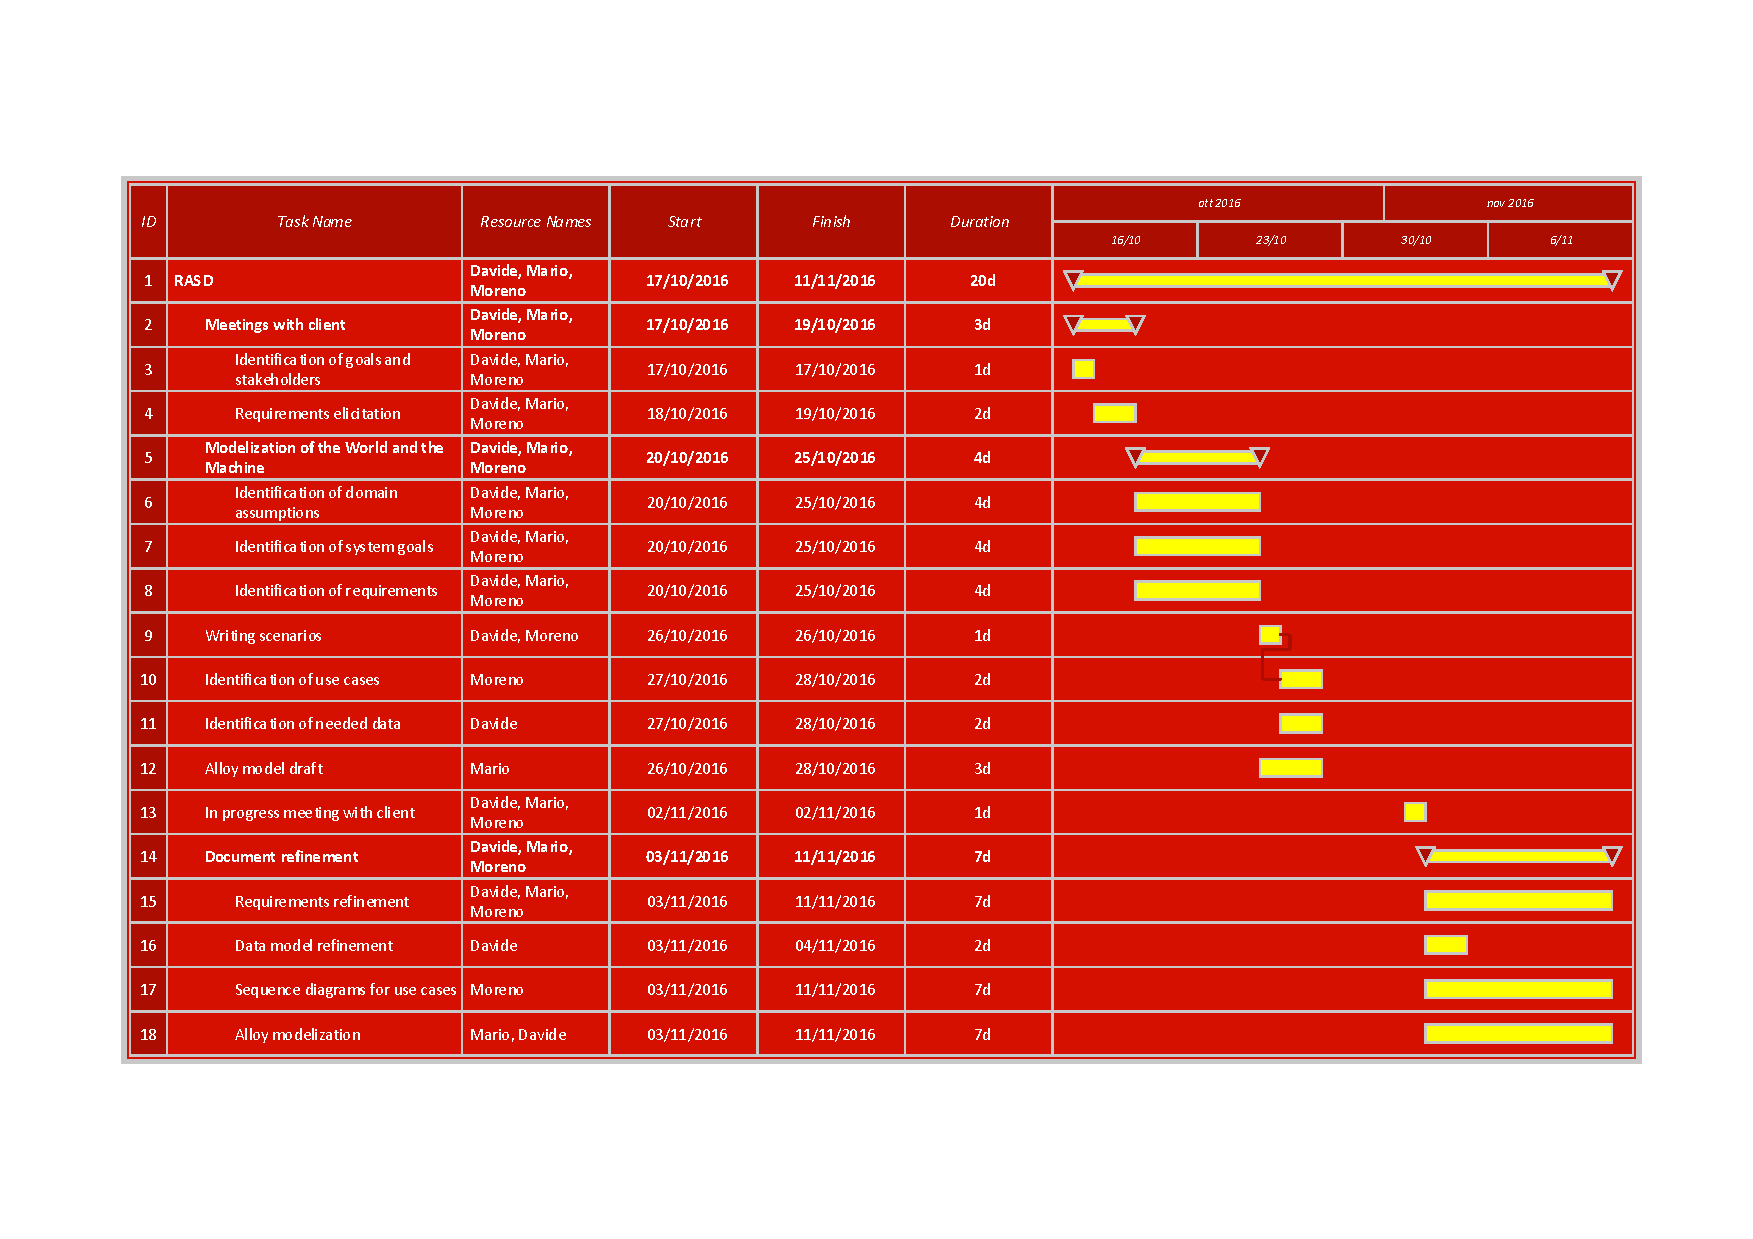
\includegraphics[angle=90, width=\linewidth]{RASDGantt}	\caption{
		\label{fig:rasdGantt} 
		RASD Gantt chart
	}
\end{figure}

\begin{figure}[h]
	\centering
	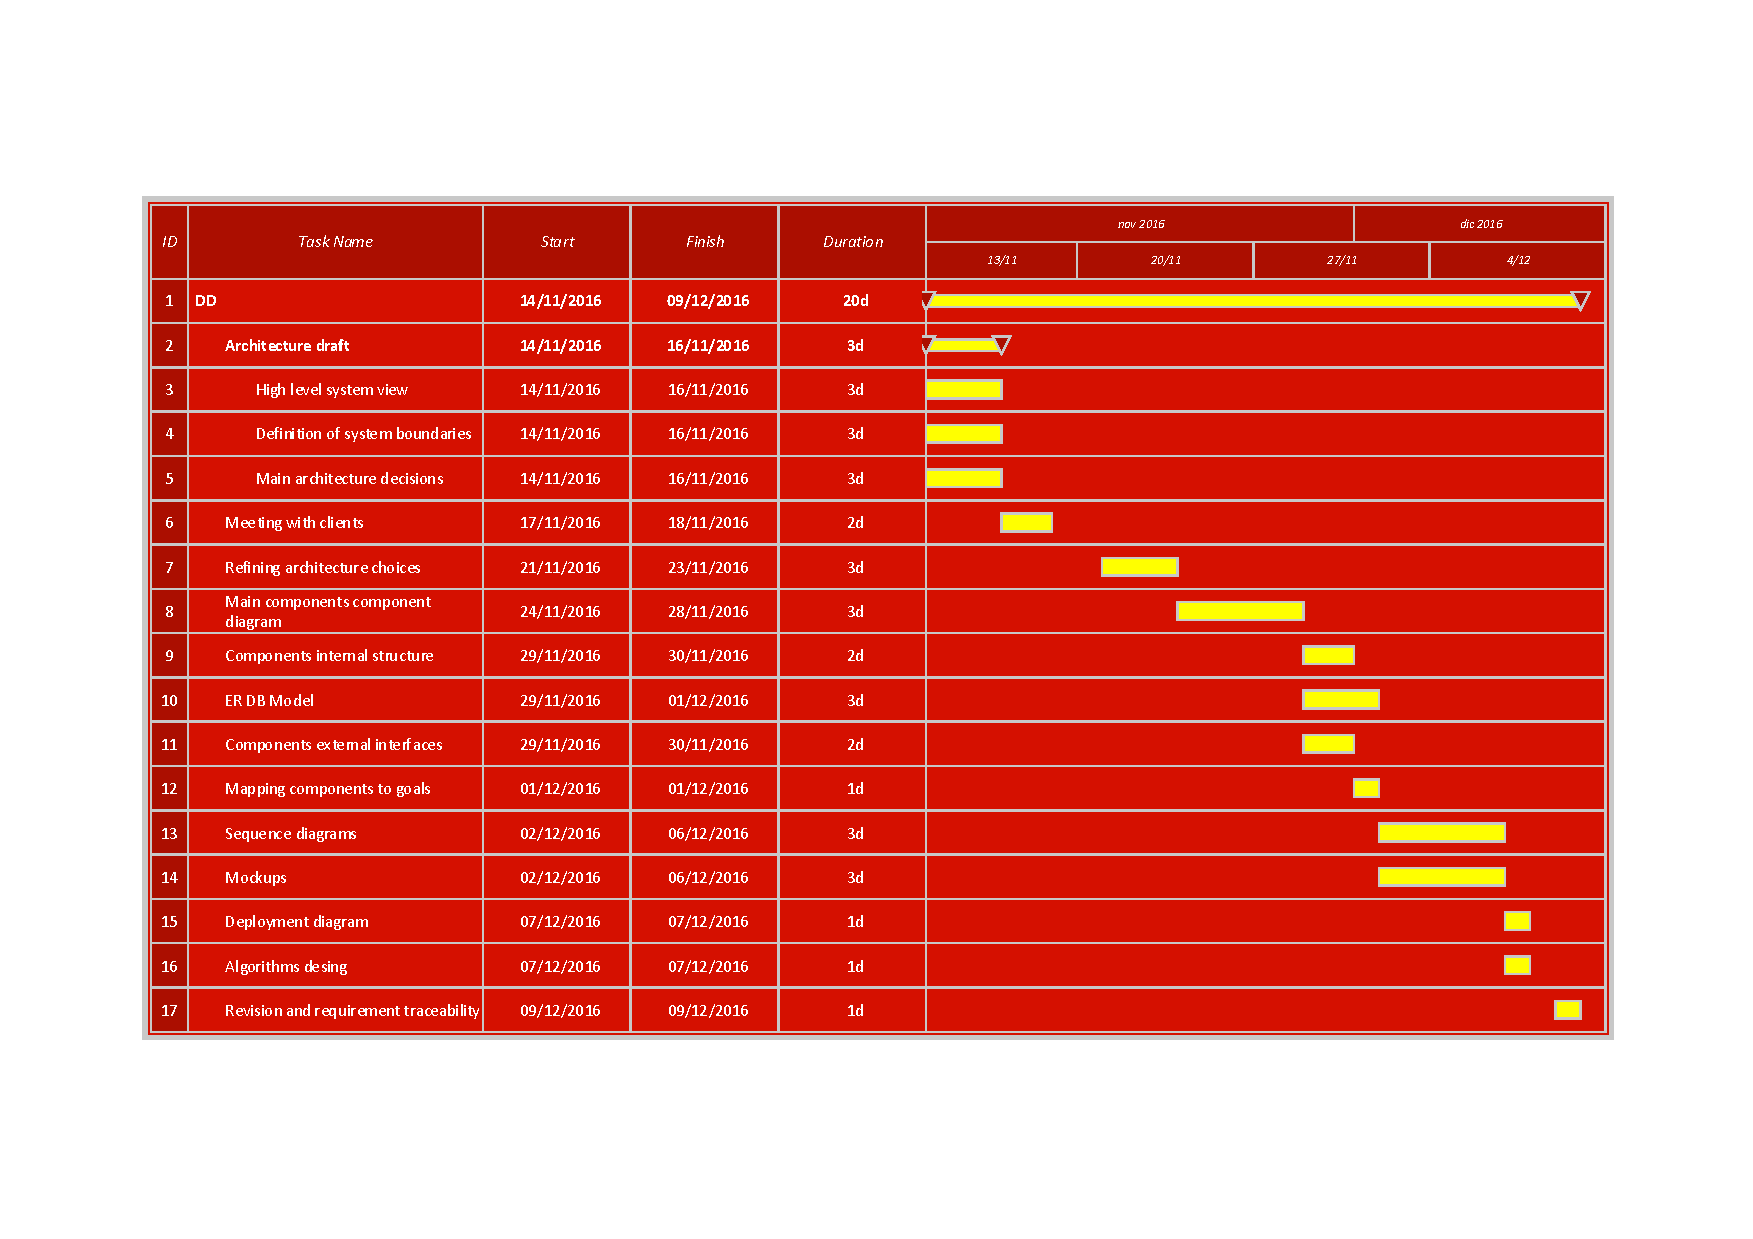
\includegraphics[angle=90, width=\linewidth]{DDGantt}	\caption{
		\label{fig:ddGantt} 
		DD Gantt chart
	}
\end{figure}

\begin{figure}[h]
	\centering
	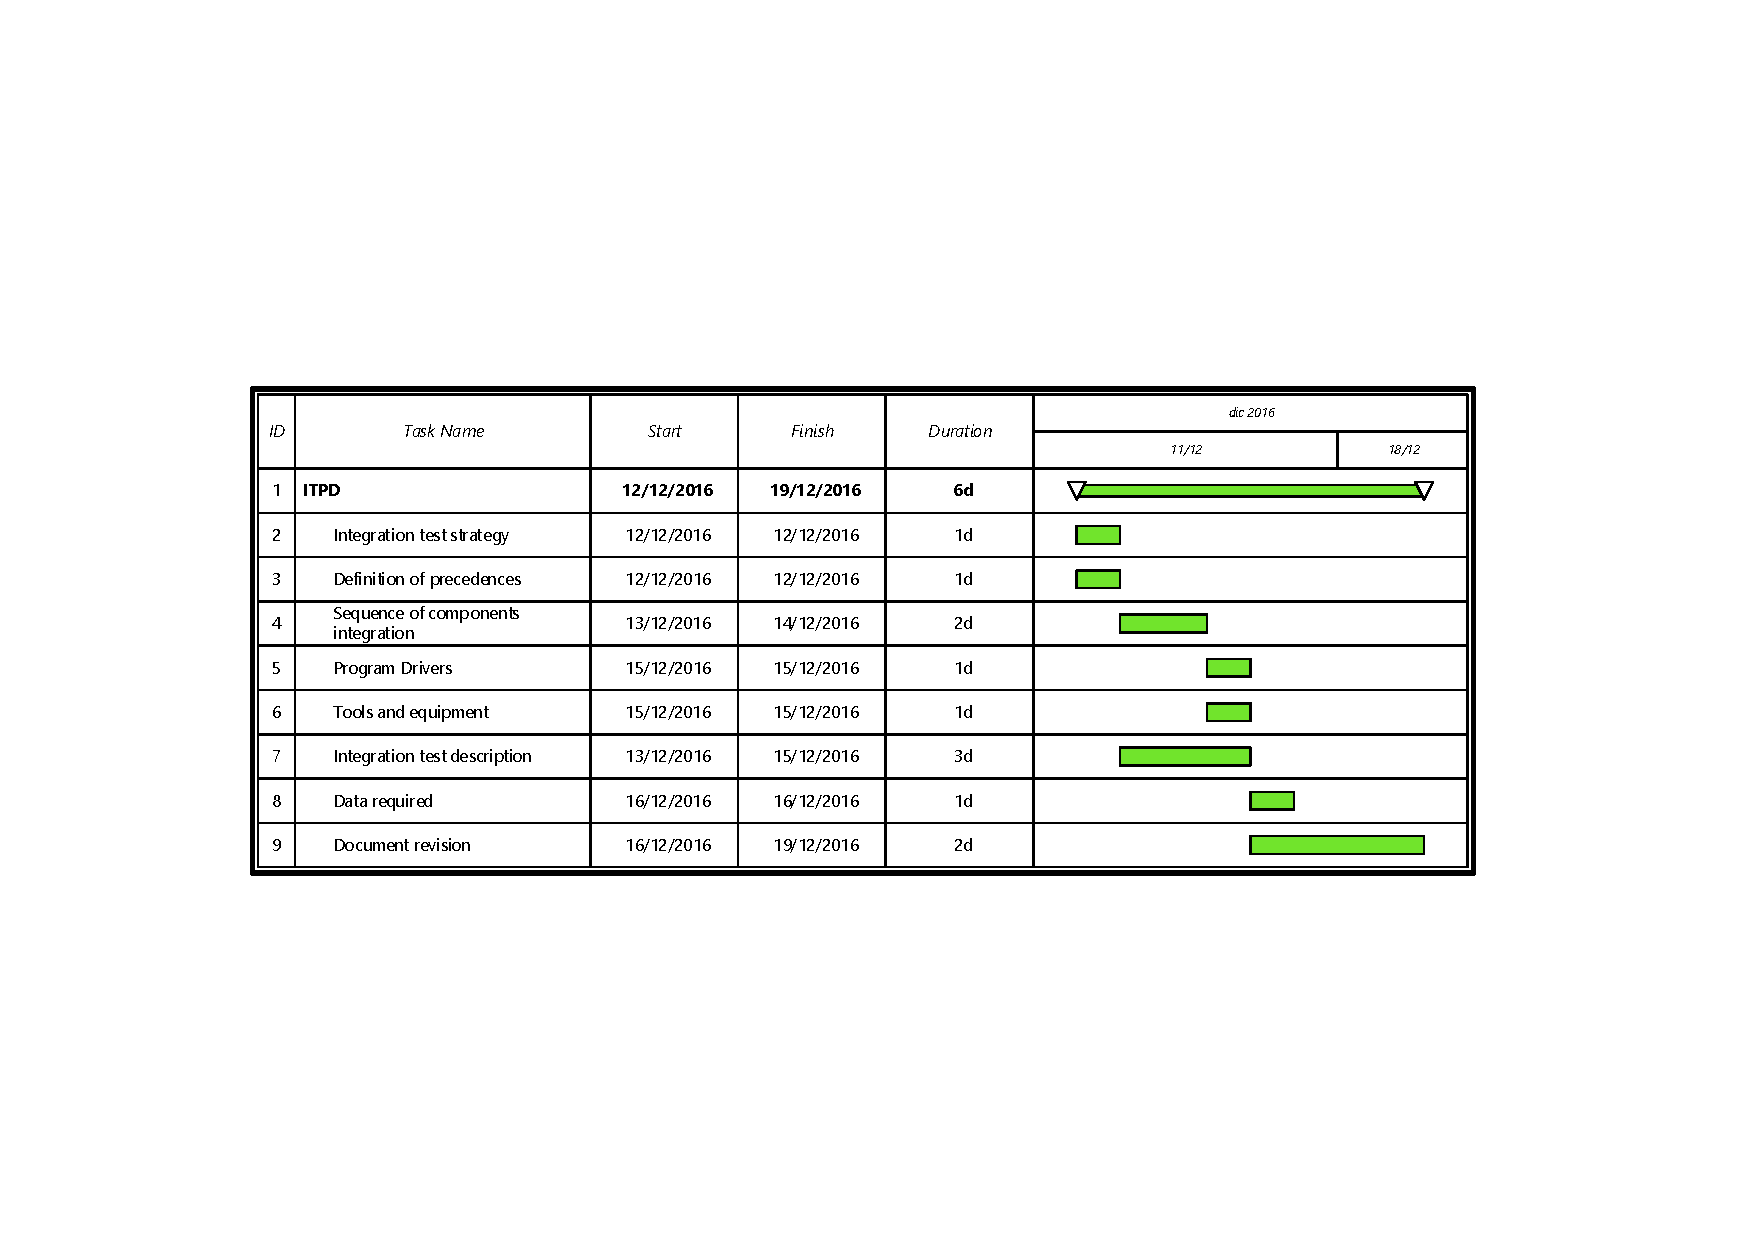
\includegraphics[angle=90, width=\linewidth]{ITPDGantt}	\caption{
		\label{fig:itpdGantt} 
		ITPD Gantt chart
	}
\end{figure}

\begin{figure}[h]
	\centering
	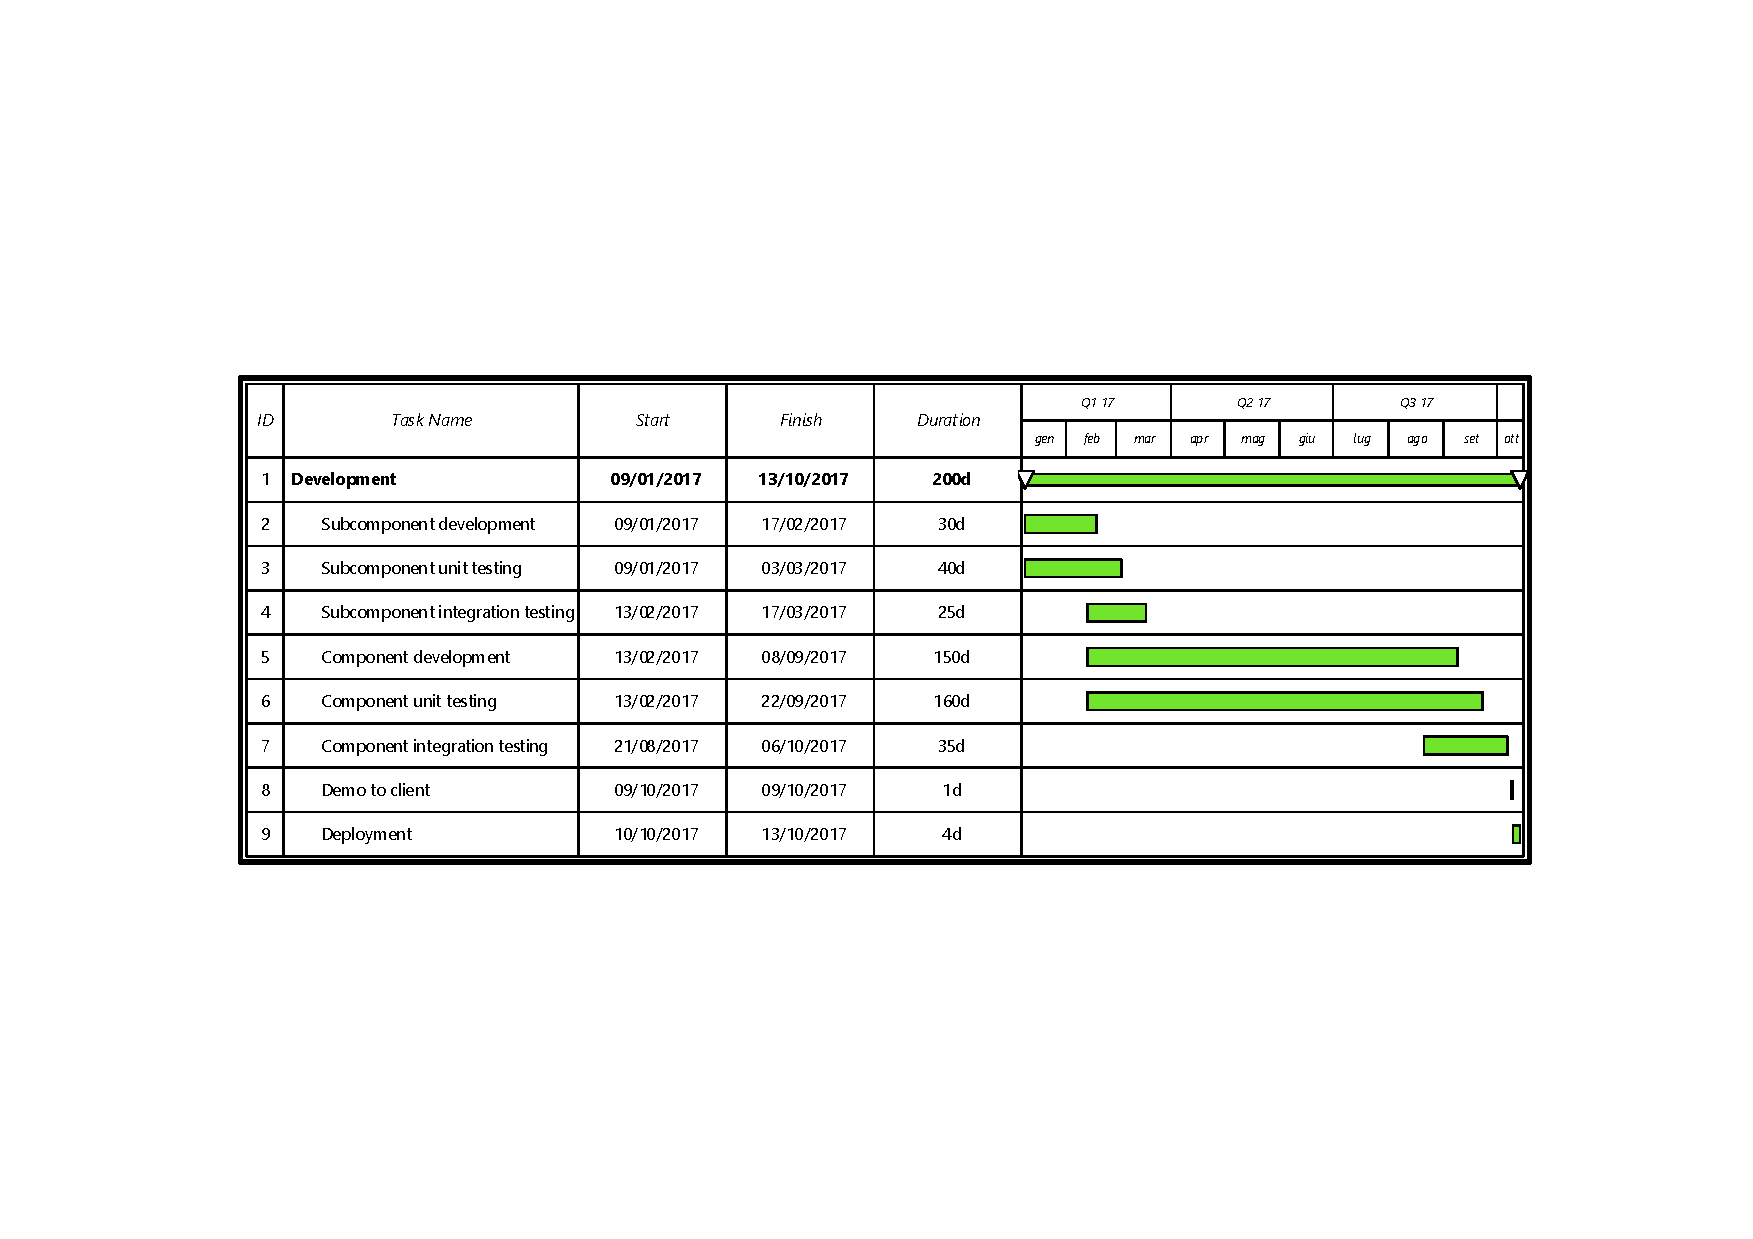
\includegraphics[angle=90, width=\linewidth]{DevGantt}	\caption{
		\label{fig:devGantt} 
		Development Gantt chart
	}
\end{figure}

\clearpage
